\documentclass[12pt]{article}
	\usepackage{setspace}
	\usepackage{graphicx}
	\usepackage{float}
	\graphicspath{{/Users/pawandeepsingh/Desktop/PR_Assignment2/My_Plots/}}

\begin{document}
	\begin{center}
		\vspace*{10mm}
		{\Huge Pattern Recognition \\}
		\vspace{5mm}
		{\huge Assignment \# 2 \\}
		\vspace{20mm}
	\end{center}
	{\large Author}: \hfill \hfill {\large Professor:} \\
	{\large Pawandeep Singh CS17S027  \hfill \hfill  Hema A. Murthy\\
		Ajay Pandey CS17S011}
	\vspace*{\fill}
	\newpage
	
	\section{Introduction}
		\subsection{Bayesian}
			\large{The Probability of finding class $ w_j$ of the object given the input feature $x$ is given by bayes formula :}\\ \par
			\large{$P(w_j | x)=\frac{P(x|w_j)P(w_j)}{P(x)}$.} \\ \par
			Assumptions : $P(x|w_j)$ is assumed to be following multi variateGaussian Distribution.
			$P(w_j)$ is  assumed to be equal for all classes.\\
			\subsection{Multi Variate Gaussian Distribution}
			As our likelihood is following multivariate gaussian distribution here is the formula for it :\\ \par
			\large{$p(x) = \frac{exp(\frac{-1(x-\mu)^T\Sigma^{-1}(x-\mu)} {2})}{(2\pi)^{d/2} |\Sigma|^{1/2}}$}\\ \par
			\subsection{Maximum Likelihood}
			We are just given the data without knowing the Covariance Matrix and mean. So we need to use training data to compute our unknown parameters $[\Sigma,\mu]$. By using maximum likelihood estimation our mean and covariance matrix are : \\ \par
			$\mu = \frac{1}{n} \sum_{k=1}^{n}x_k$ \\ \par
			$\Sigma = \frac{1}{n} \sum_{k=1}^{n}(x_k - \mu)(x_k - \mu)^t$
			\newpage

 	\section{Gaussian surface and contour plots}
	\begin{figure}[H]
			\begin{minipage}{0.97\textwidth}
				\centering
				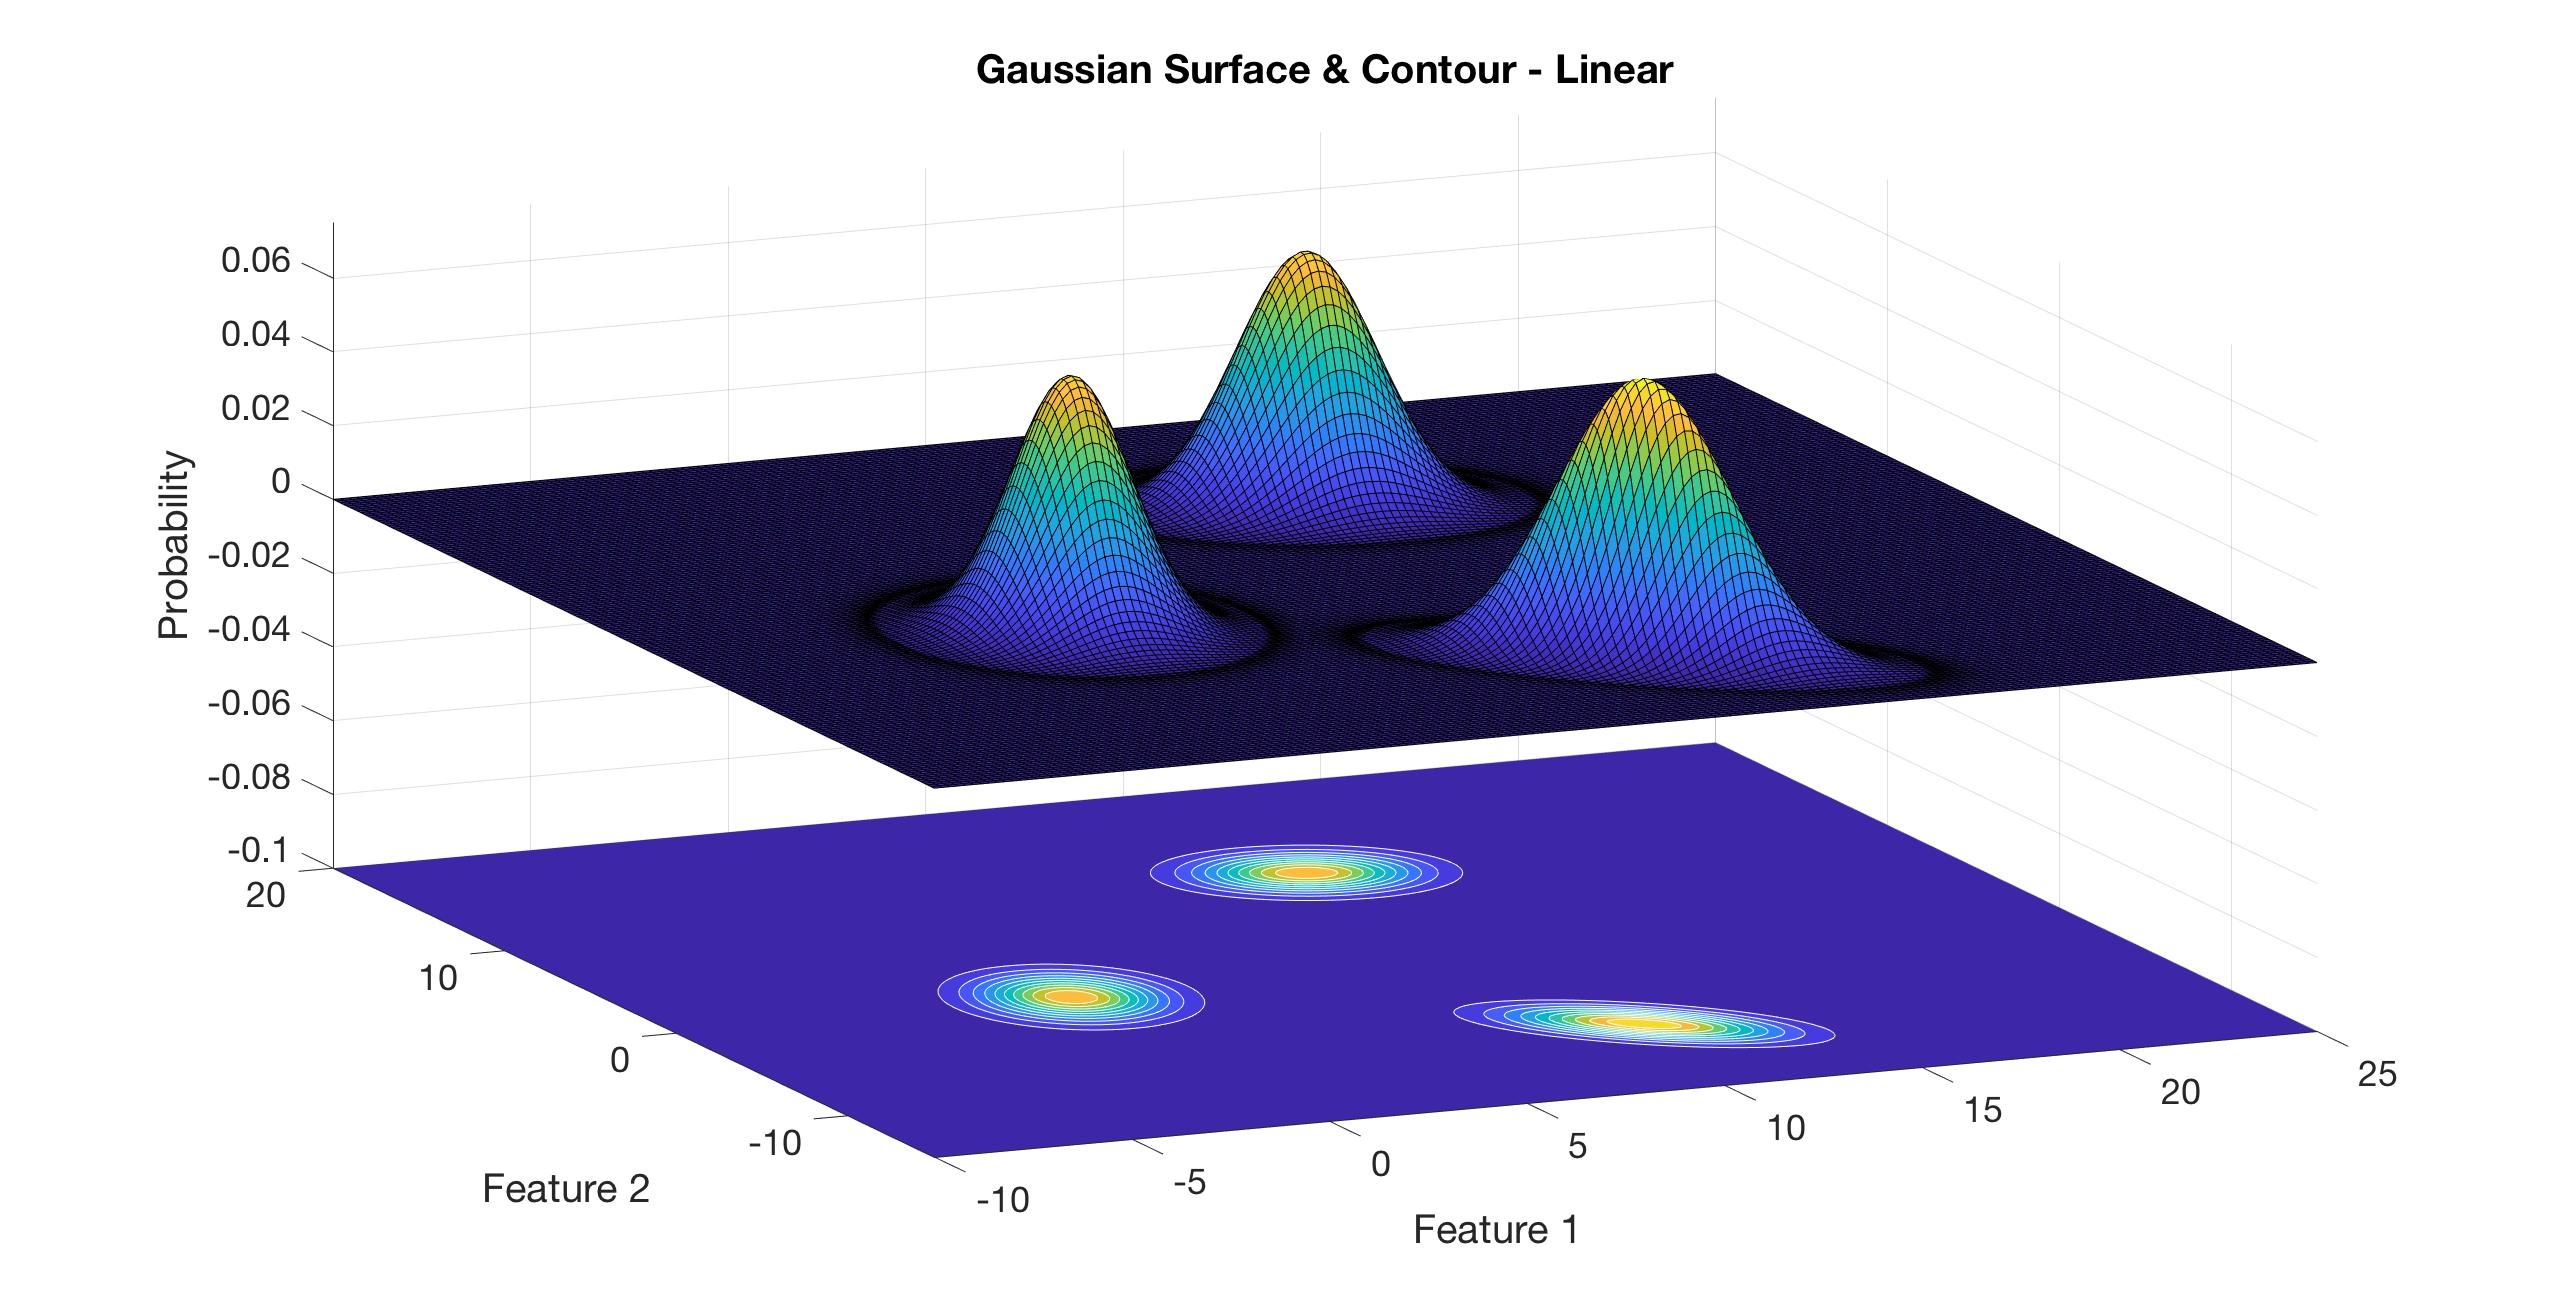
\includegraphics[width=1.0\linewidth]{gaussian_surface_linear.jpg}
			\end{minipage}\hfill
			\begin{minipage}{0.97\textwidth}
				\centering
				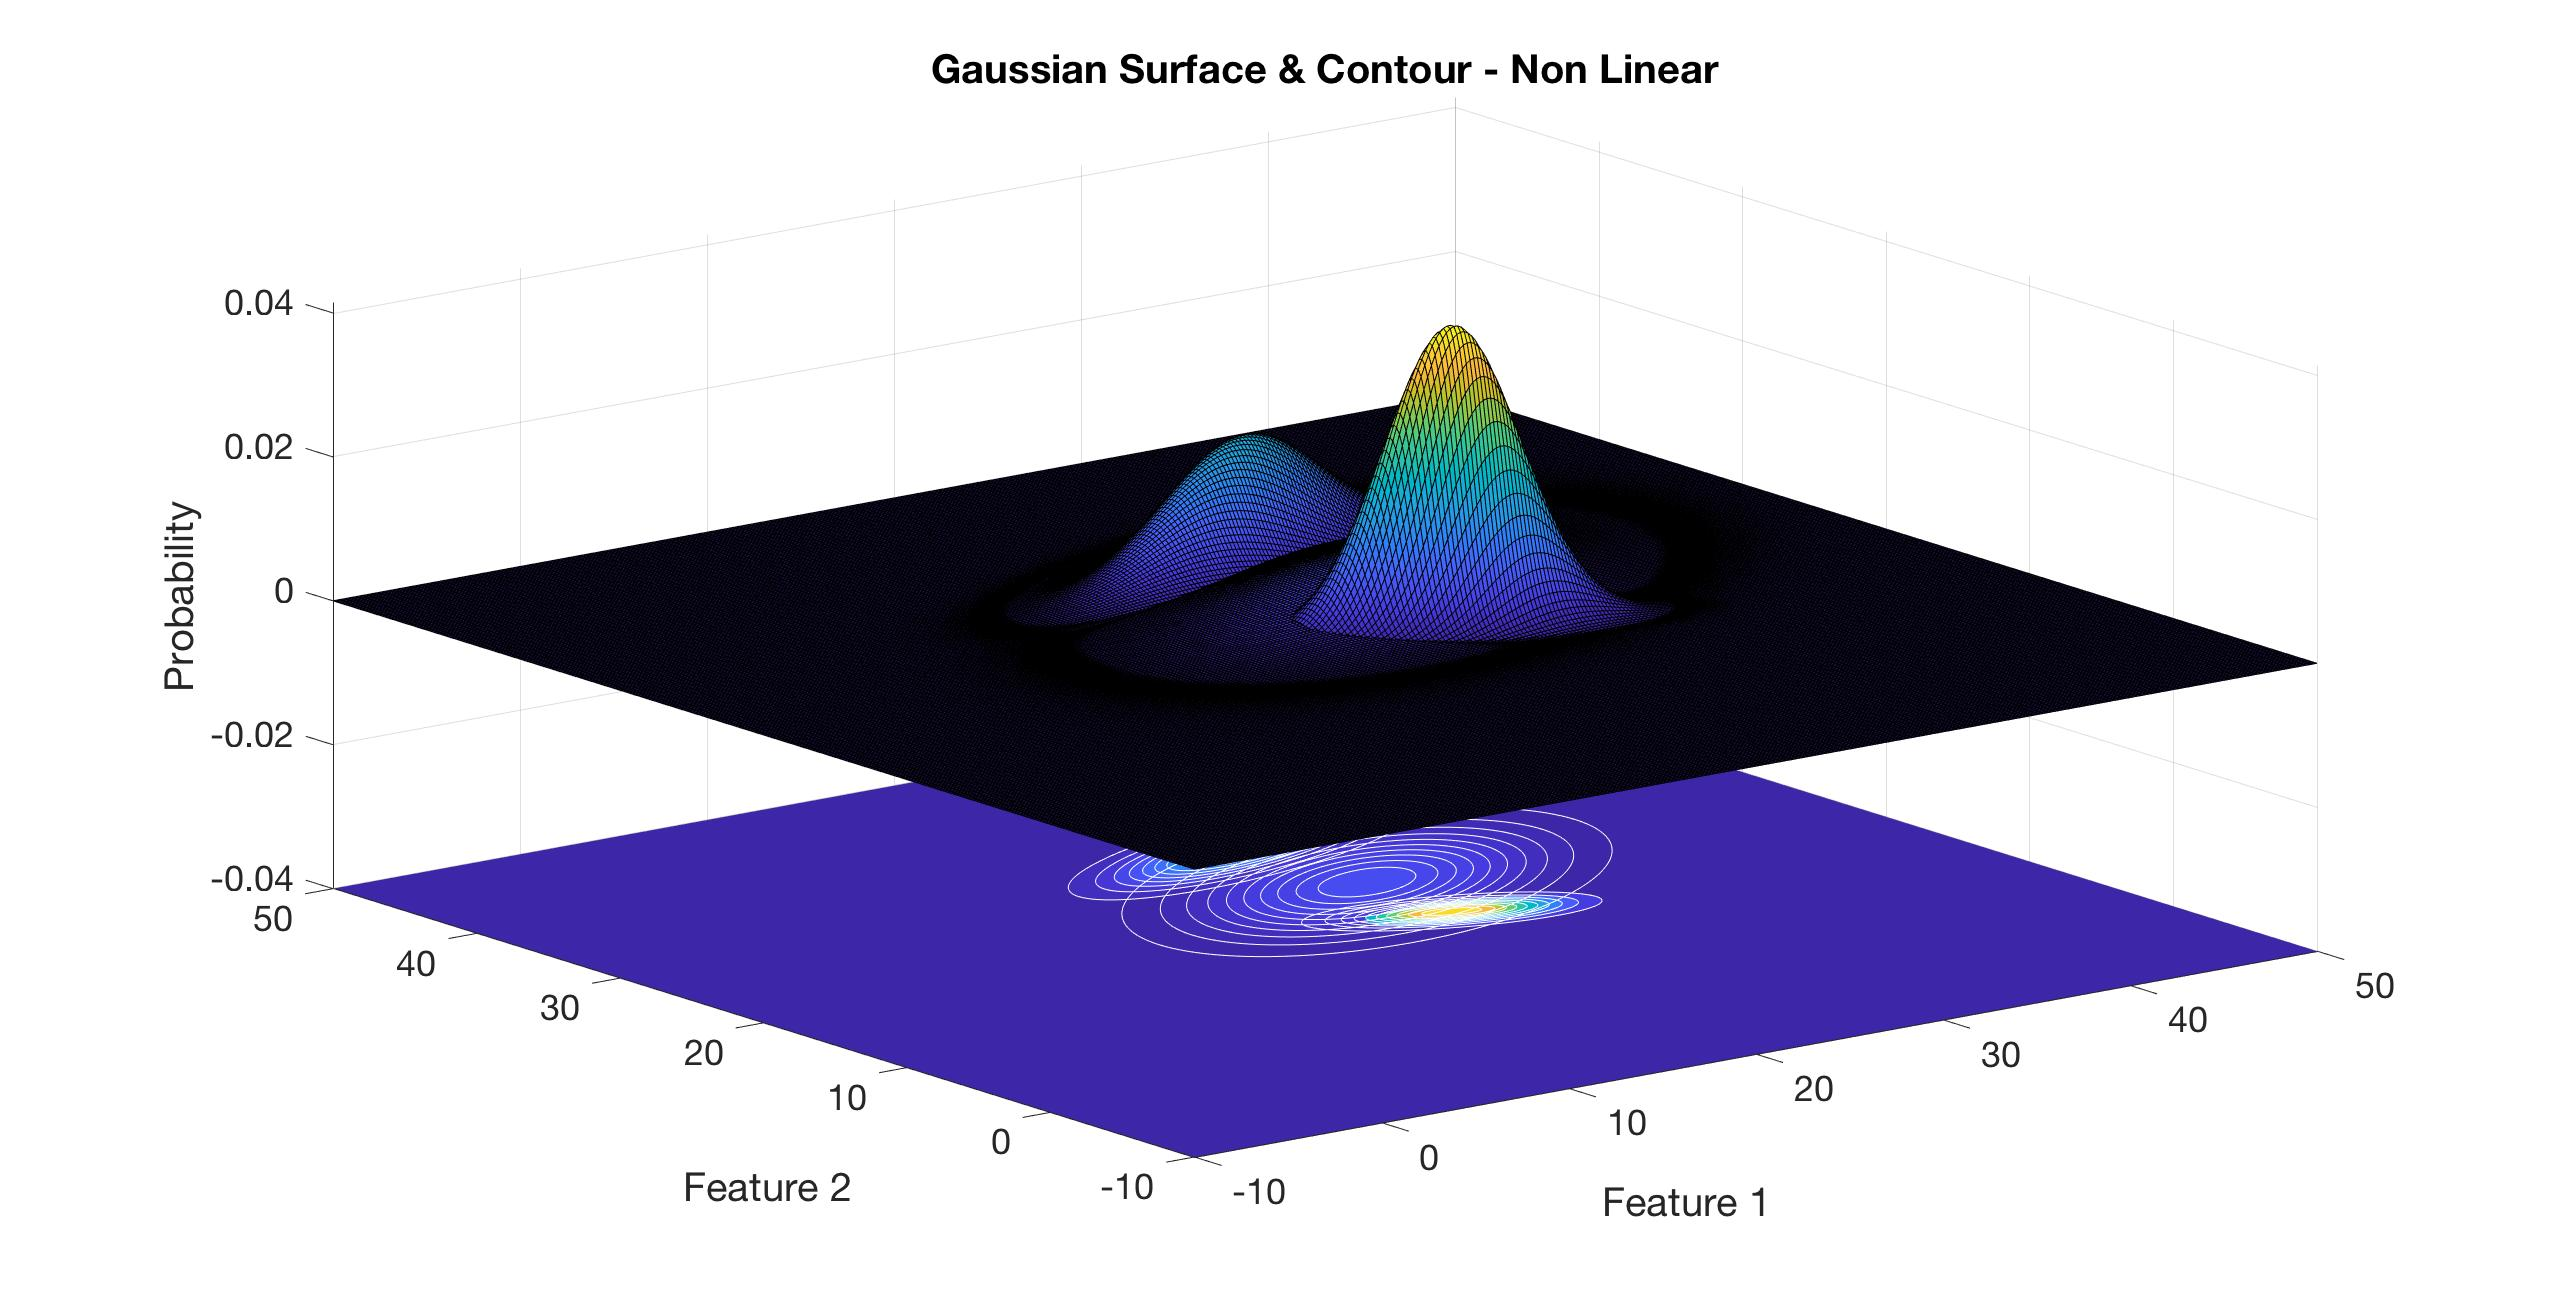
\includegraphics[width=1.0\linewidth]{gaussian_surface_non_lin.jpg}
			\end{minipage}
			\begin{minipage}{0.97\textwidth}
				\centering
				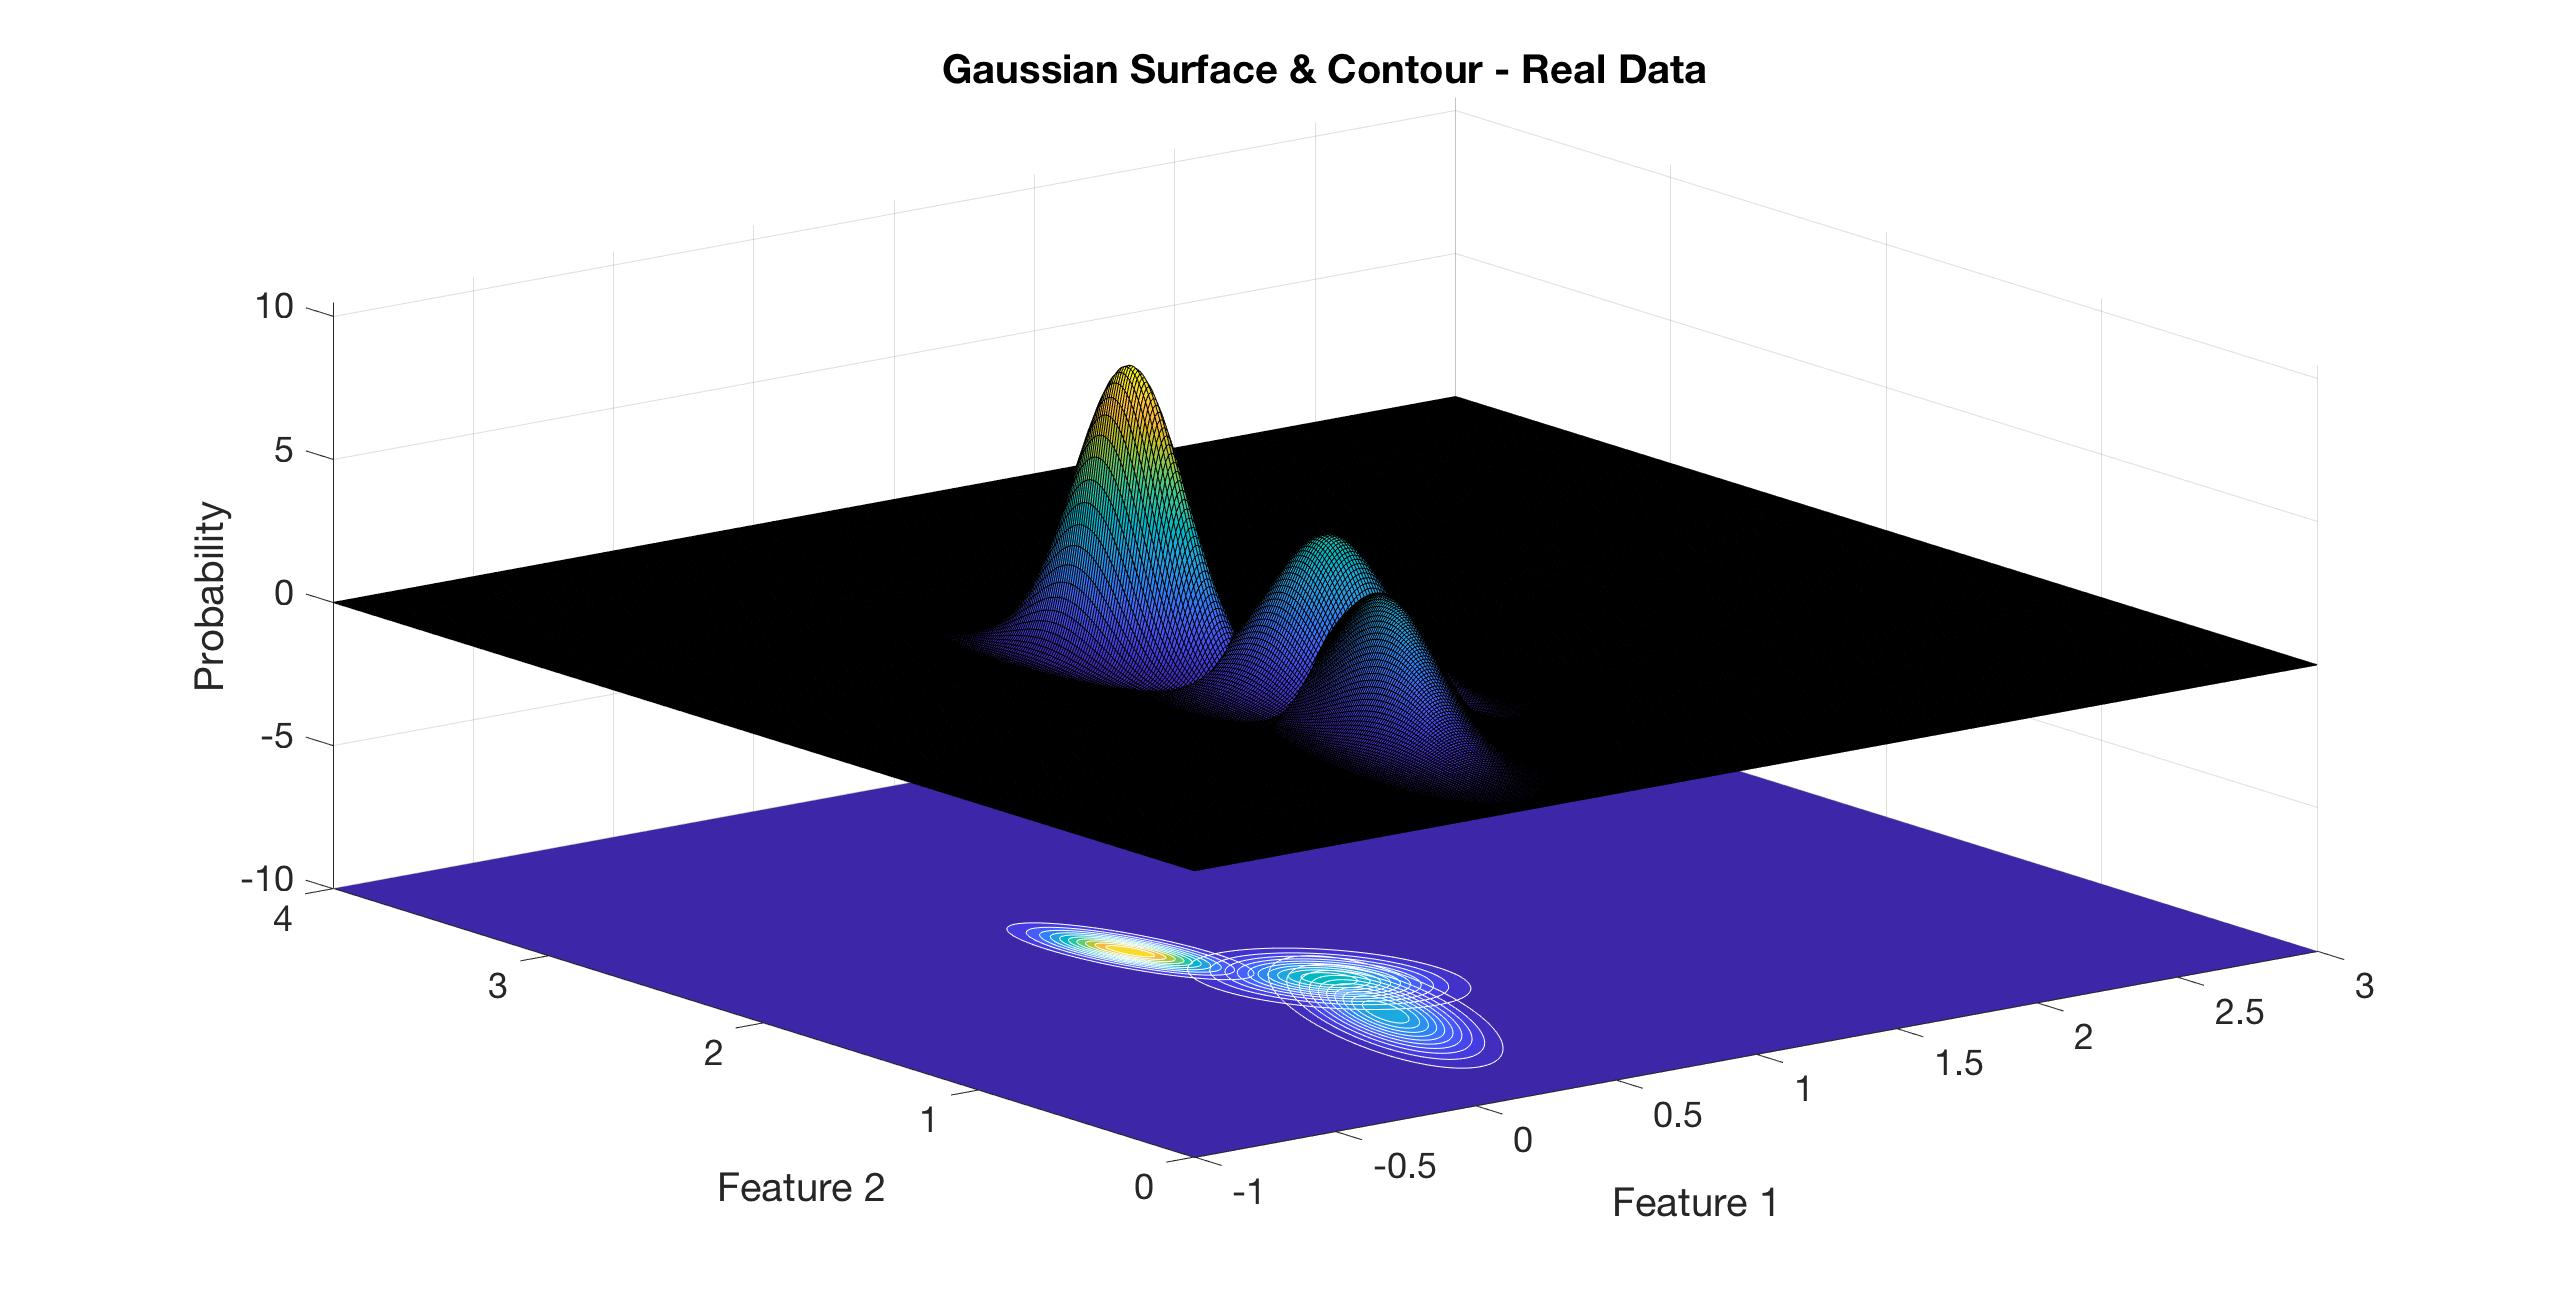
\includegraphics[width=1.0\linewidth]{gaussian_surface_real.jpg}
			\end{minipage}
	\end{figure}\newpage

	\section{Constant Density Curve and Eigen Vectors}
	\begin{figure}[H]
		\begin{minipage}{1.0\textwidth}
			\centering
			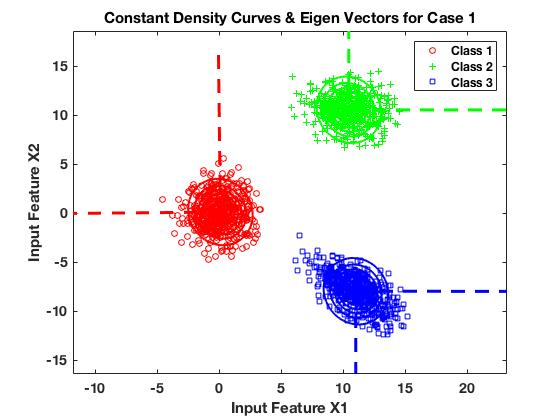
\includegraphics[width=0.5\linewidth]{LS_Contours_Case_1.jpg}
		\end{minipage}\hfill
		\begin{minipage}{1.0\textwidth}
			\centering
			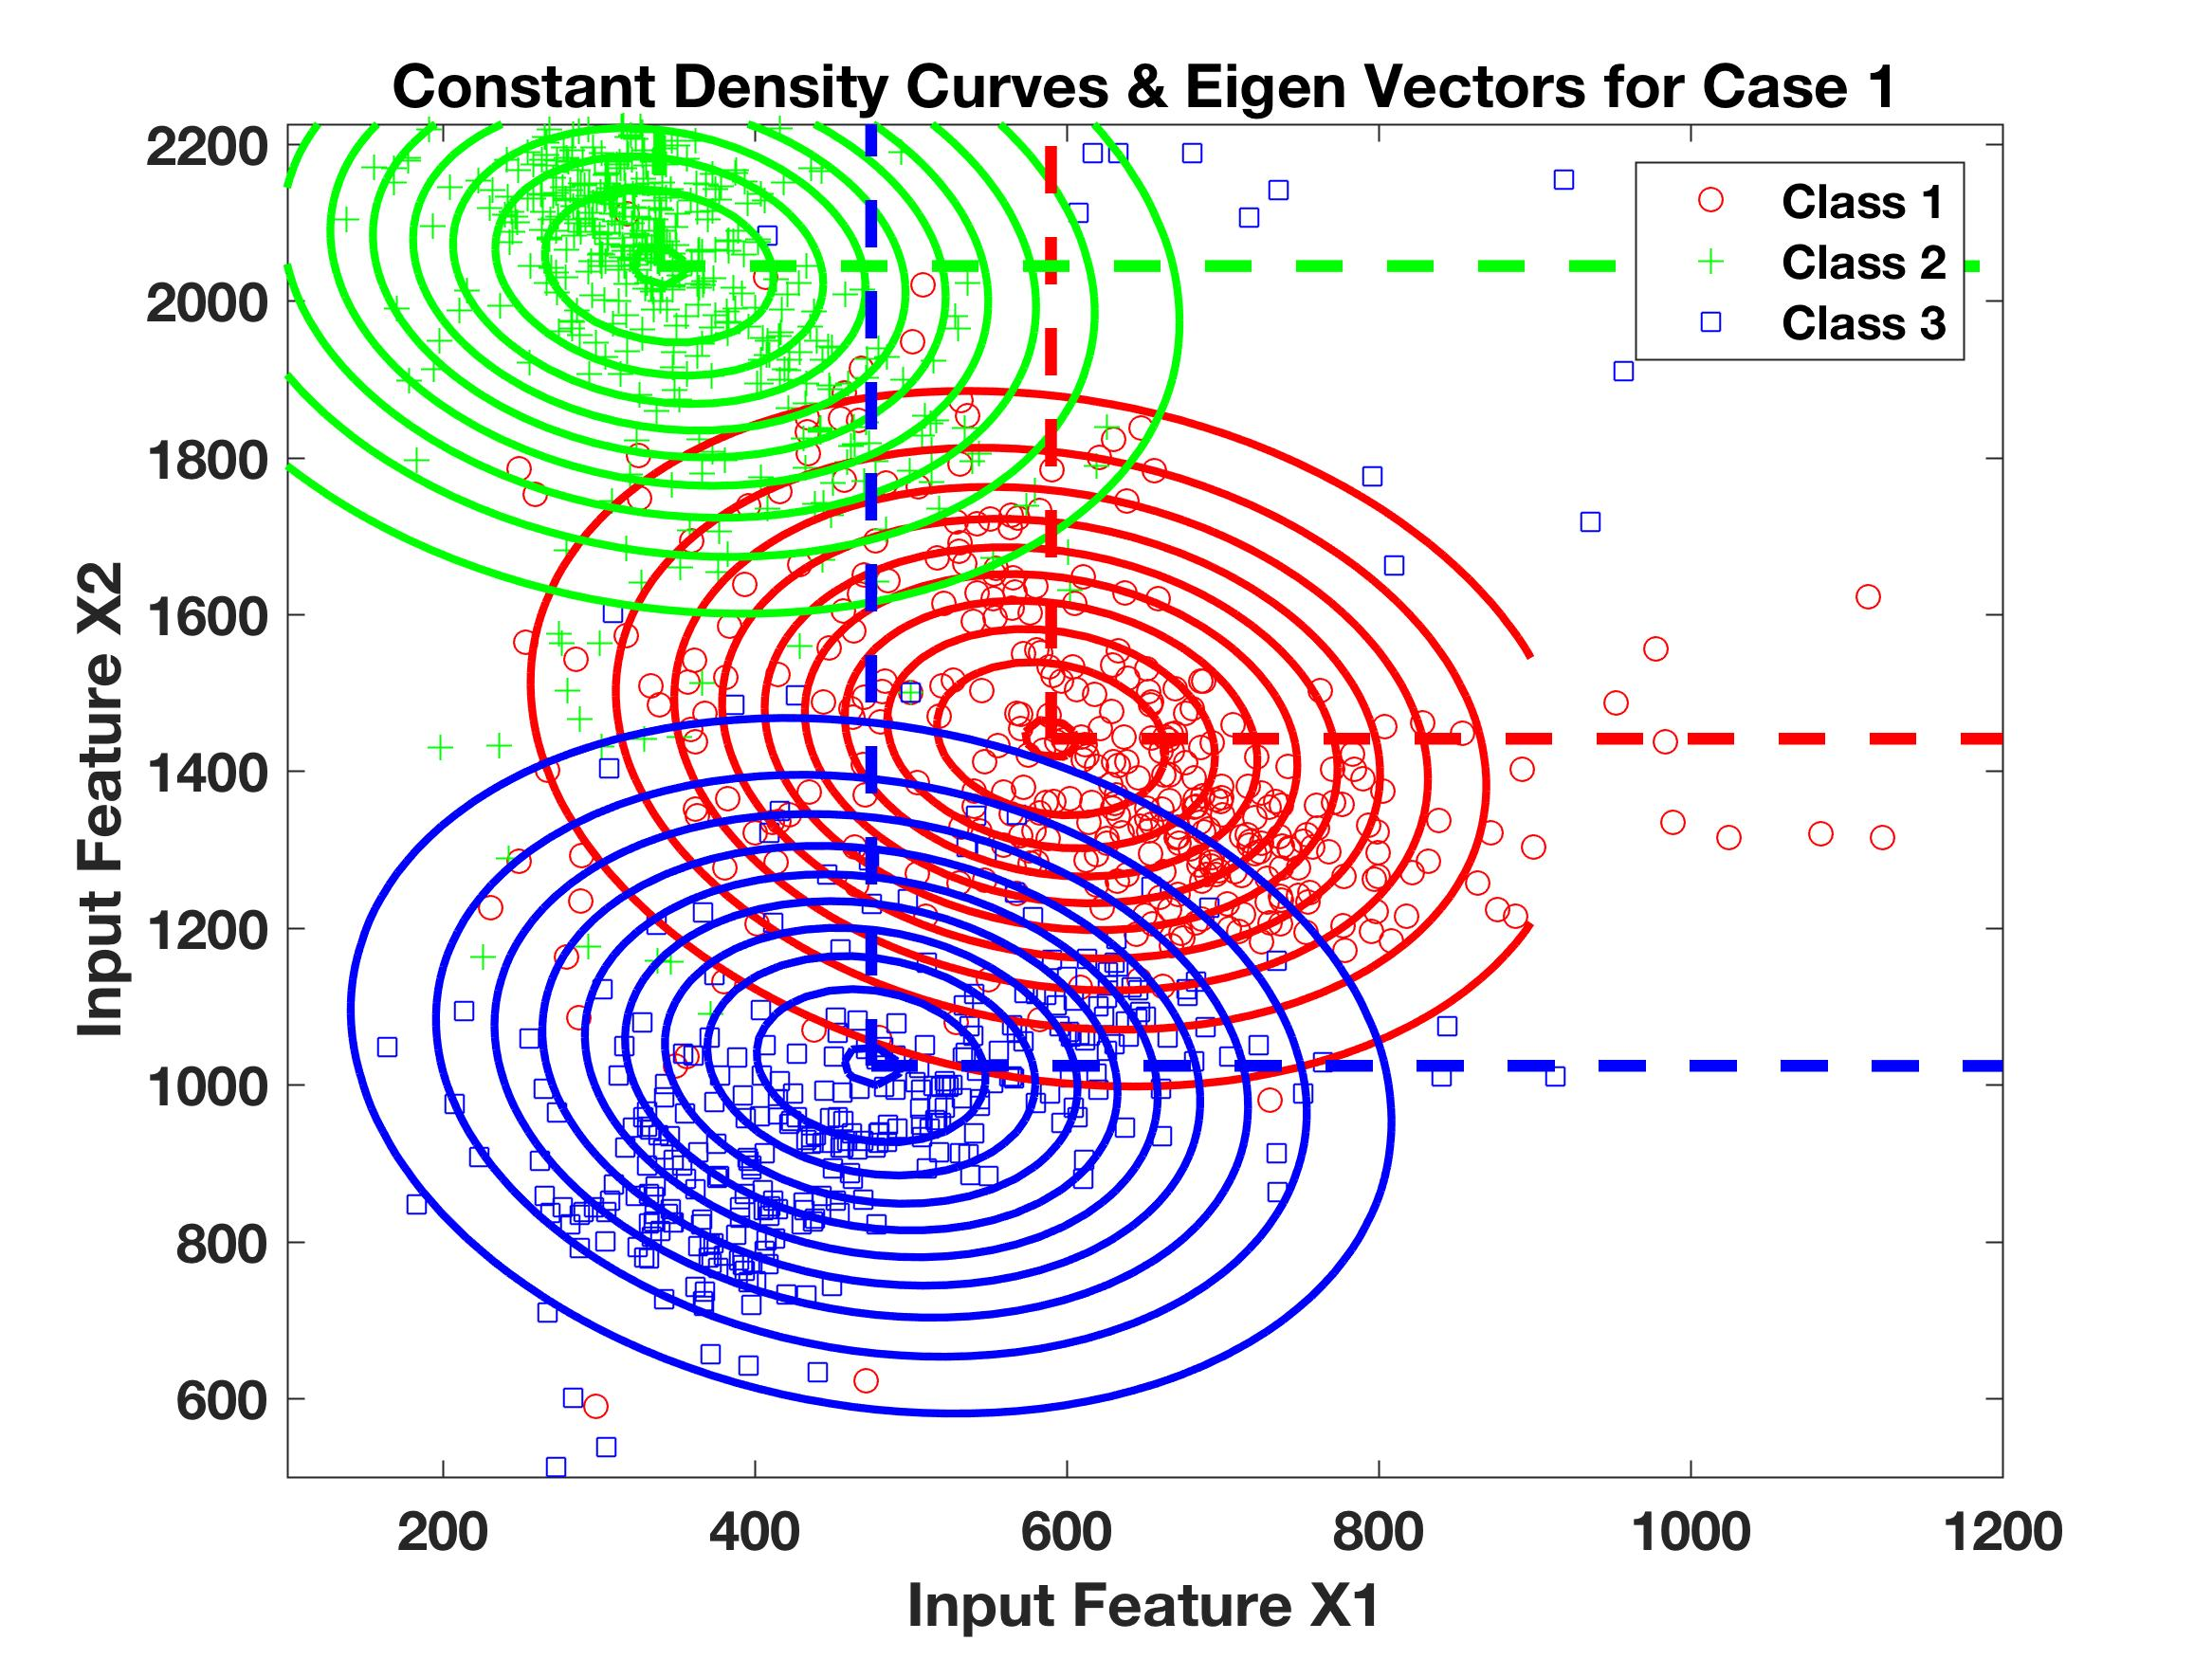
\includegraphics[width=0.5\linewidth]{RD_Contours_Case_1.jpg}
		\end{minipage}
		\begin{minipage}{1.0\textwidth}
			\centering
			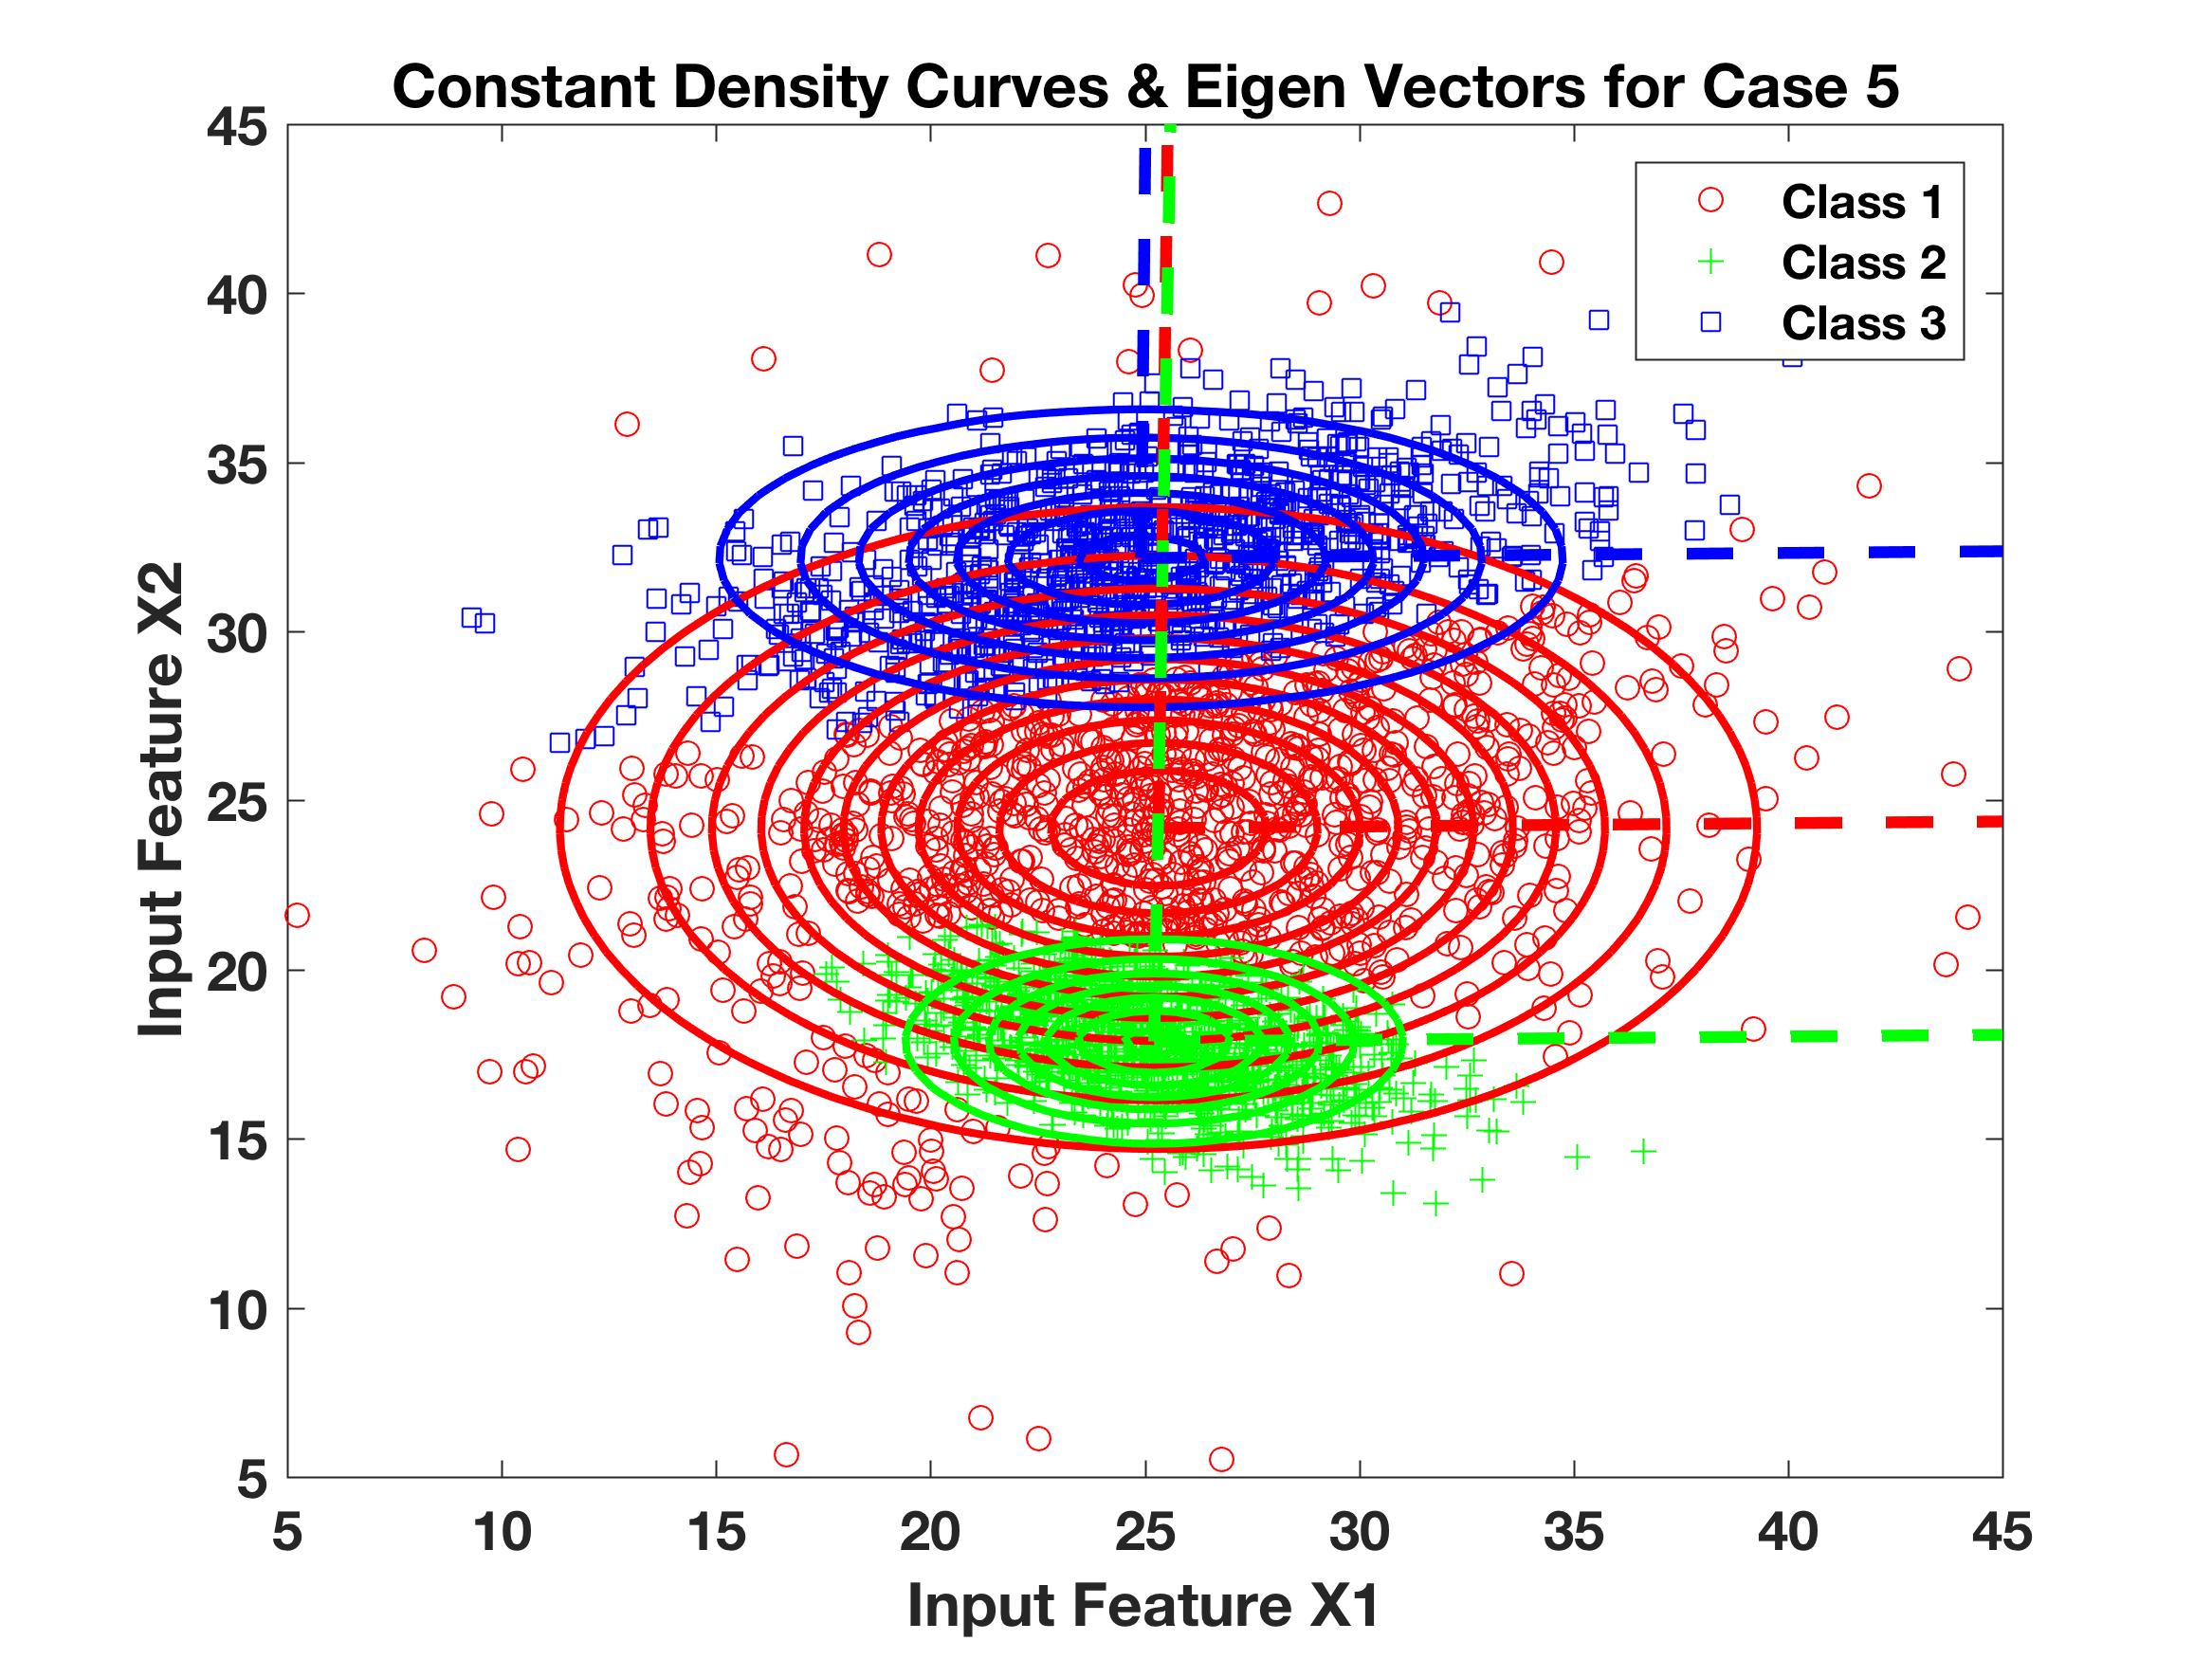
\includegraphics[width=0.5\linewidth]{NLS_Contours_Case_5.jpg}
		\end{minipage}
		\end{figure}
			Constant density curves form concentric circles when covariance of all the classes are same and eclipse otherwise.	
	\newpage
	
		\section{Confusion Matrix}
	\begin{figure}[H]
		\begin{minipage}{1.0\textwidth}
			\centering
			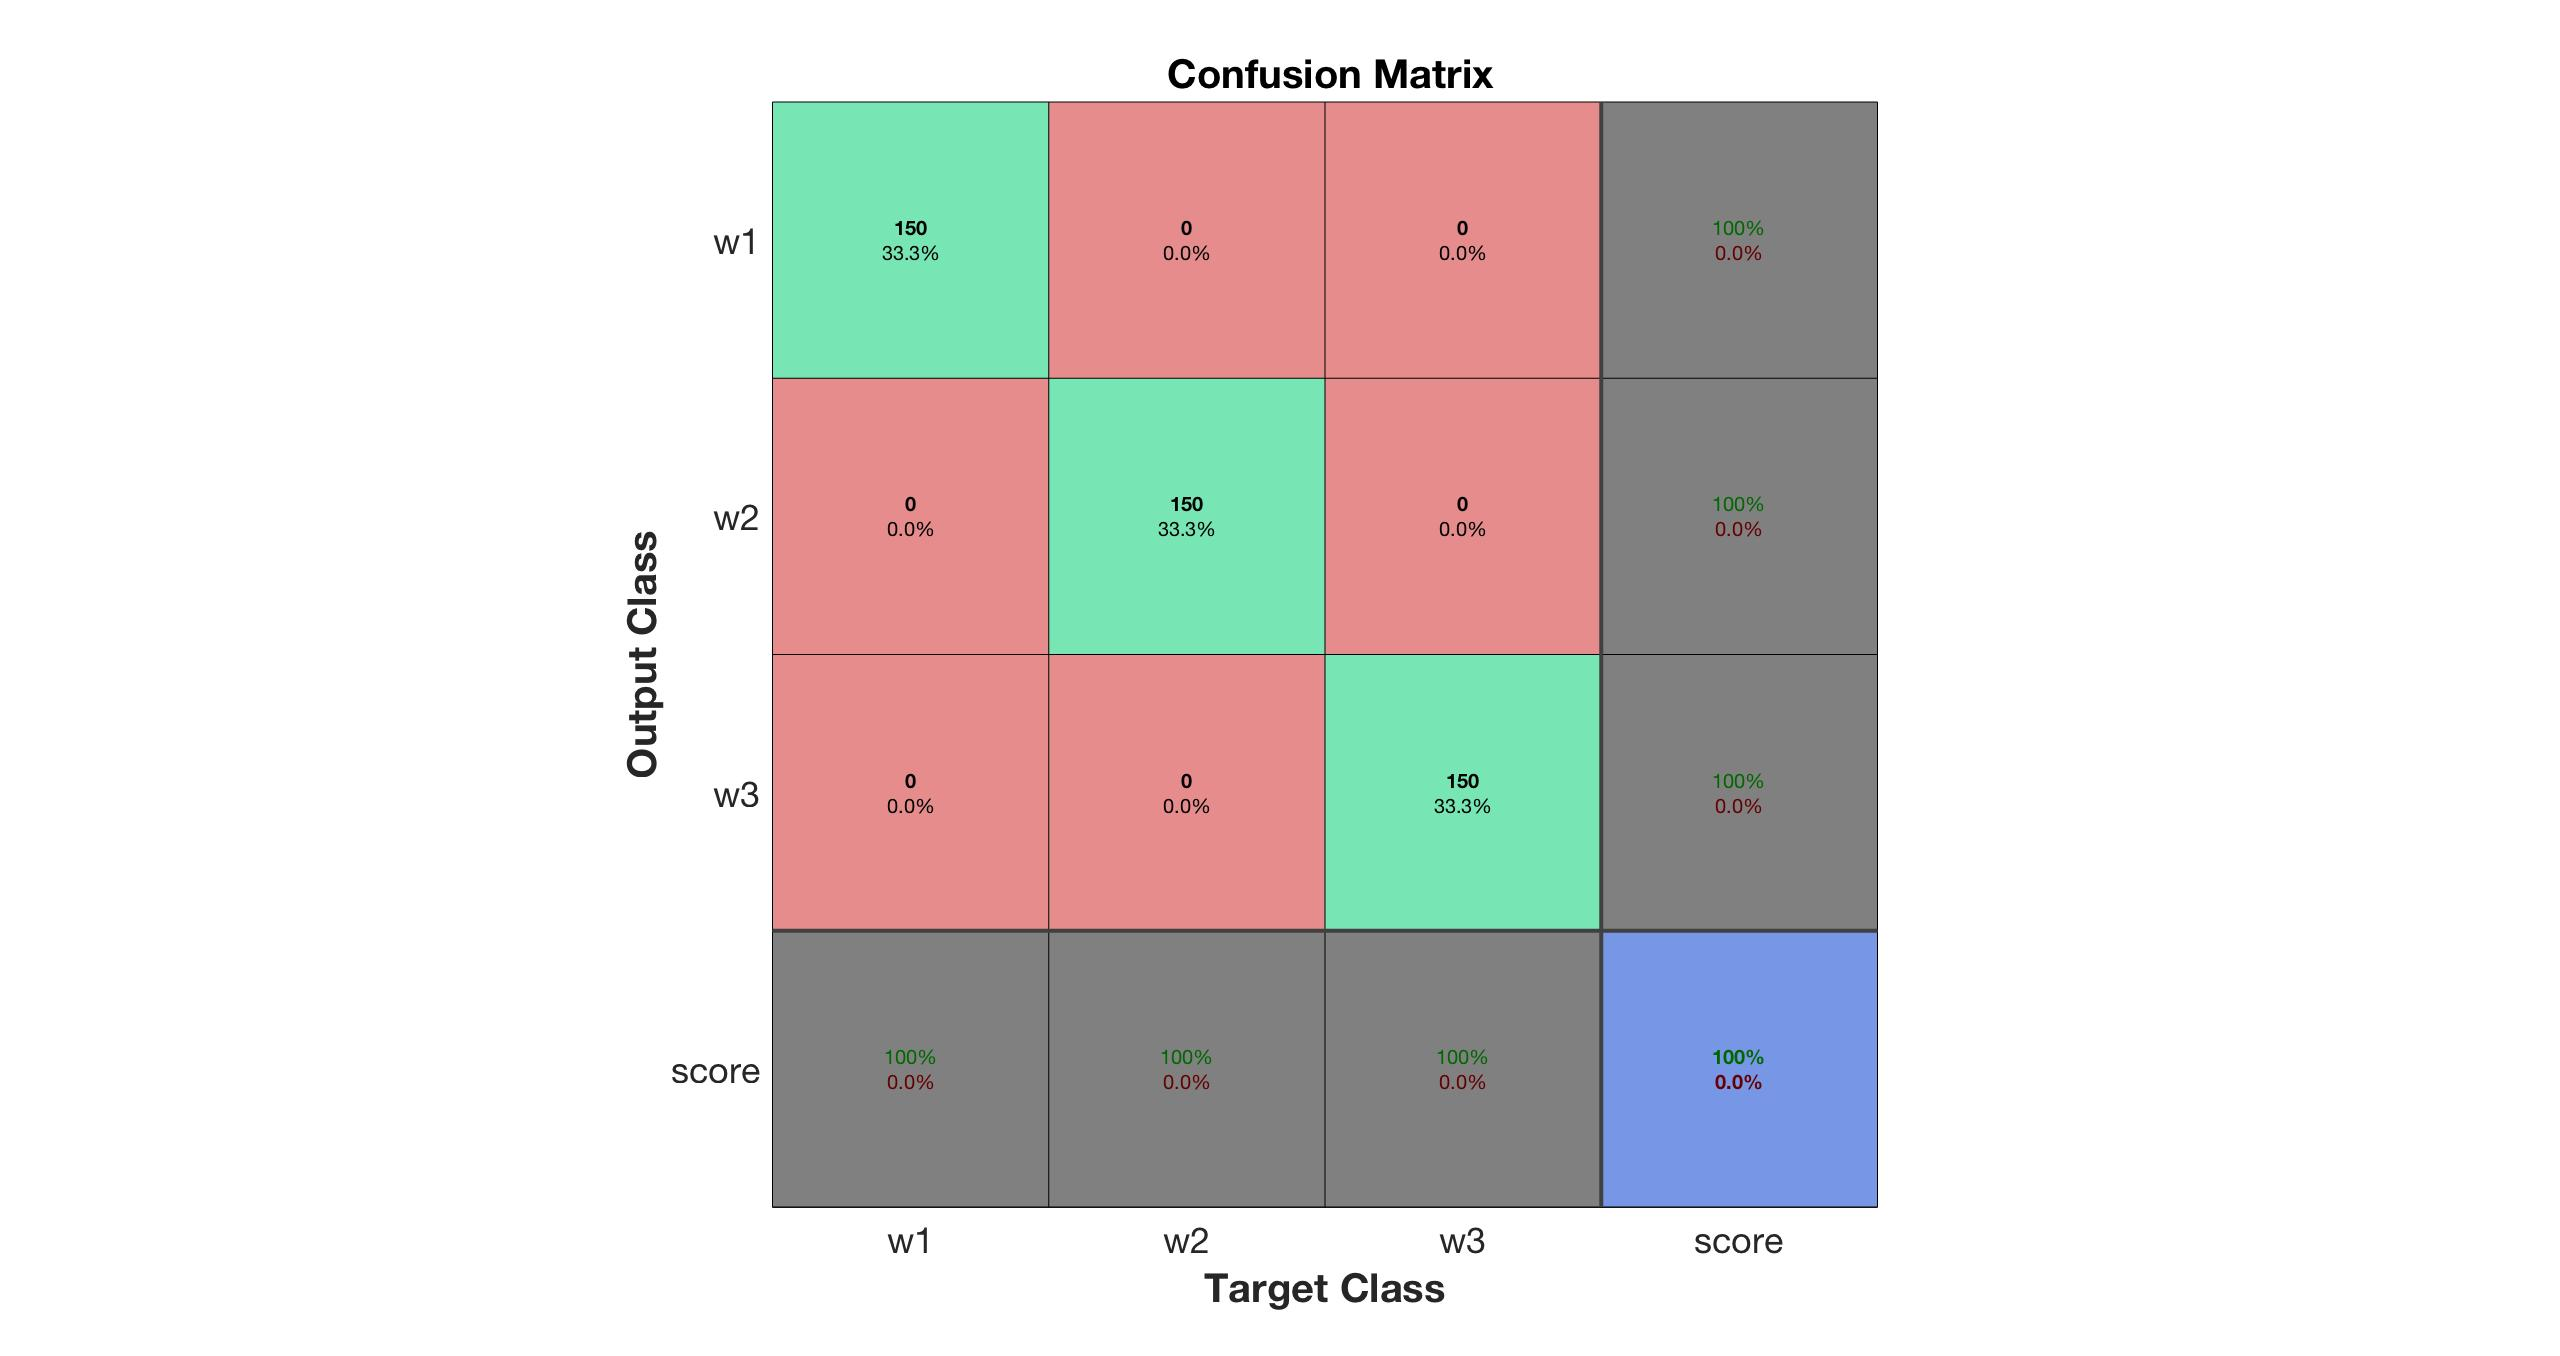
\includegraphics[width=1.0\linewidth]{confusion_matrix_linear_cov_same.jpg}
		\end{minipage}\hfill
		\begin{minipage}{1.0\textwidth}
			\centering
			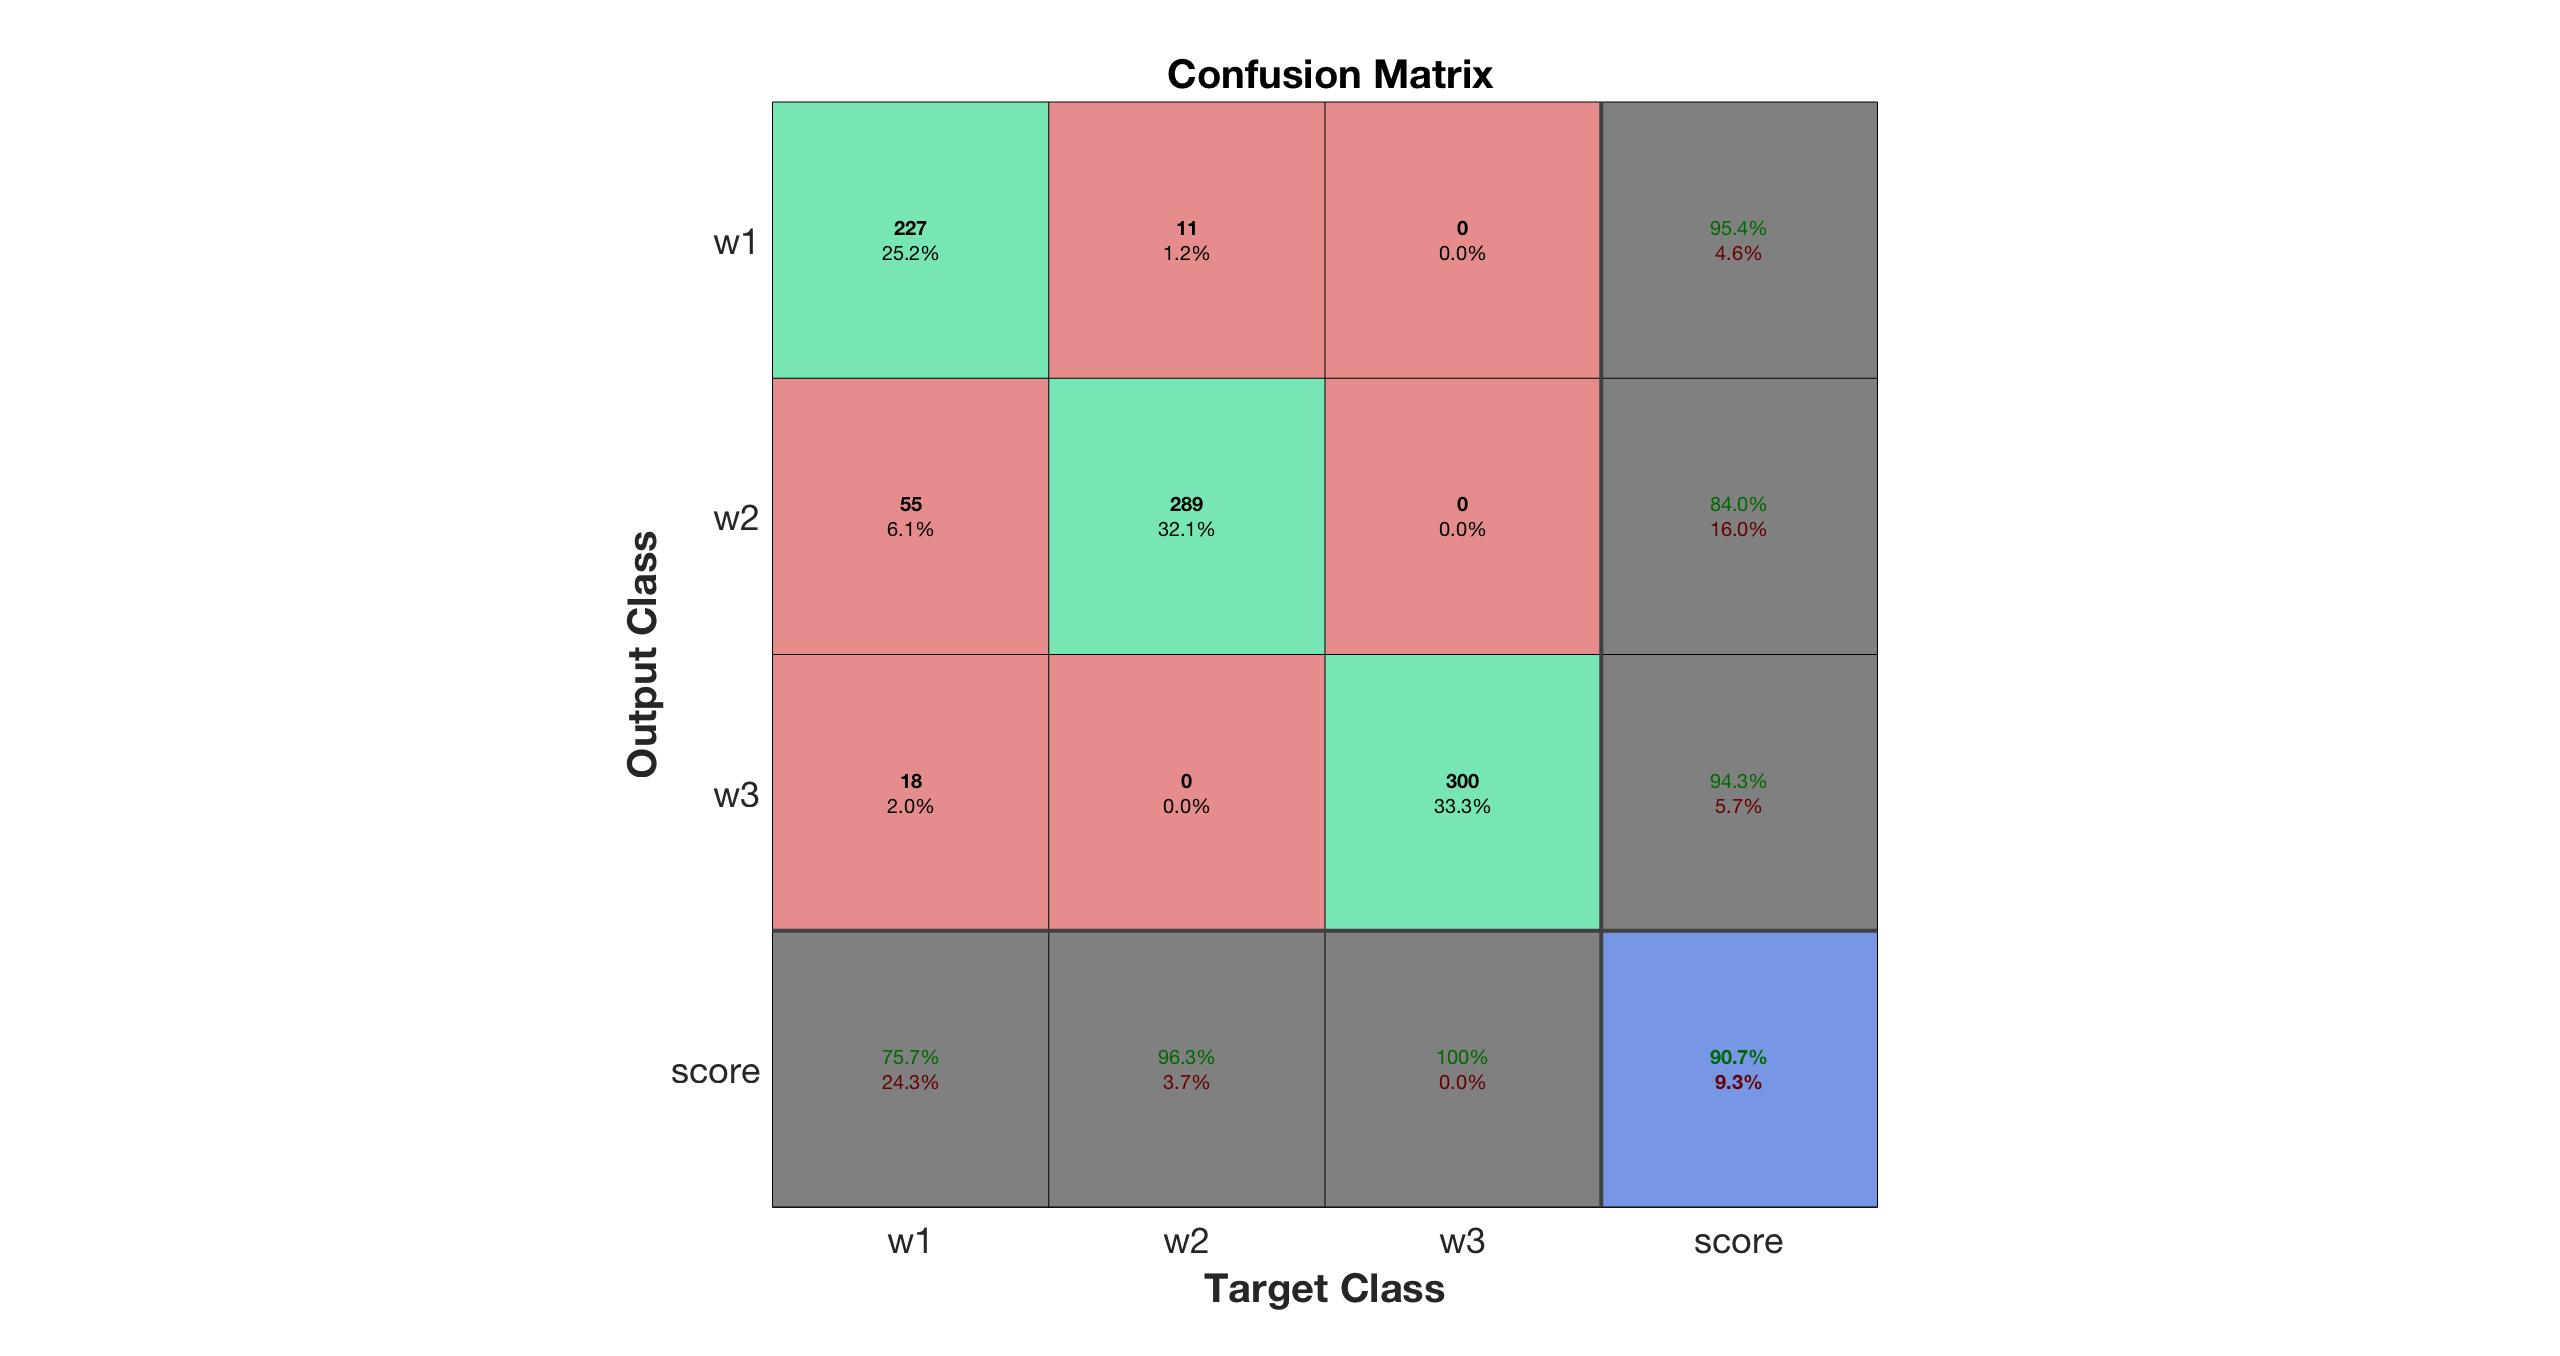
\includegraphics[width=1.0\linewidth]{confusion_matrix_non_linear_cov_same.jpg}
		\end{minipage}
	\end{figure}
	Confusion matrix display how our model is working on a certain threshold. For linear seperable data, our bayes model gives $100\%$ accuracy while it decreases as our data gets more complex. High accuracy in confusion matrix mean higher \% along diagonal.
	\newpage
	
		\section{Reciever Operating Characteristics}
	\begin{figure}[H]
		\begin{minipage}{1.0\textwidth}
			\centering
			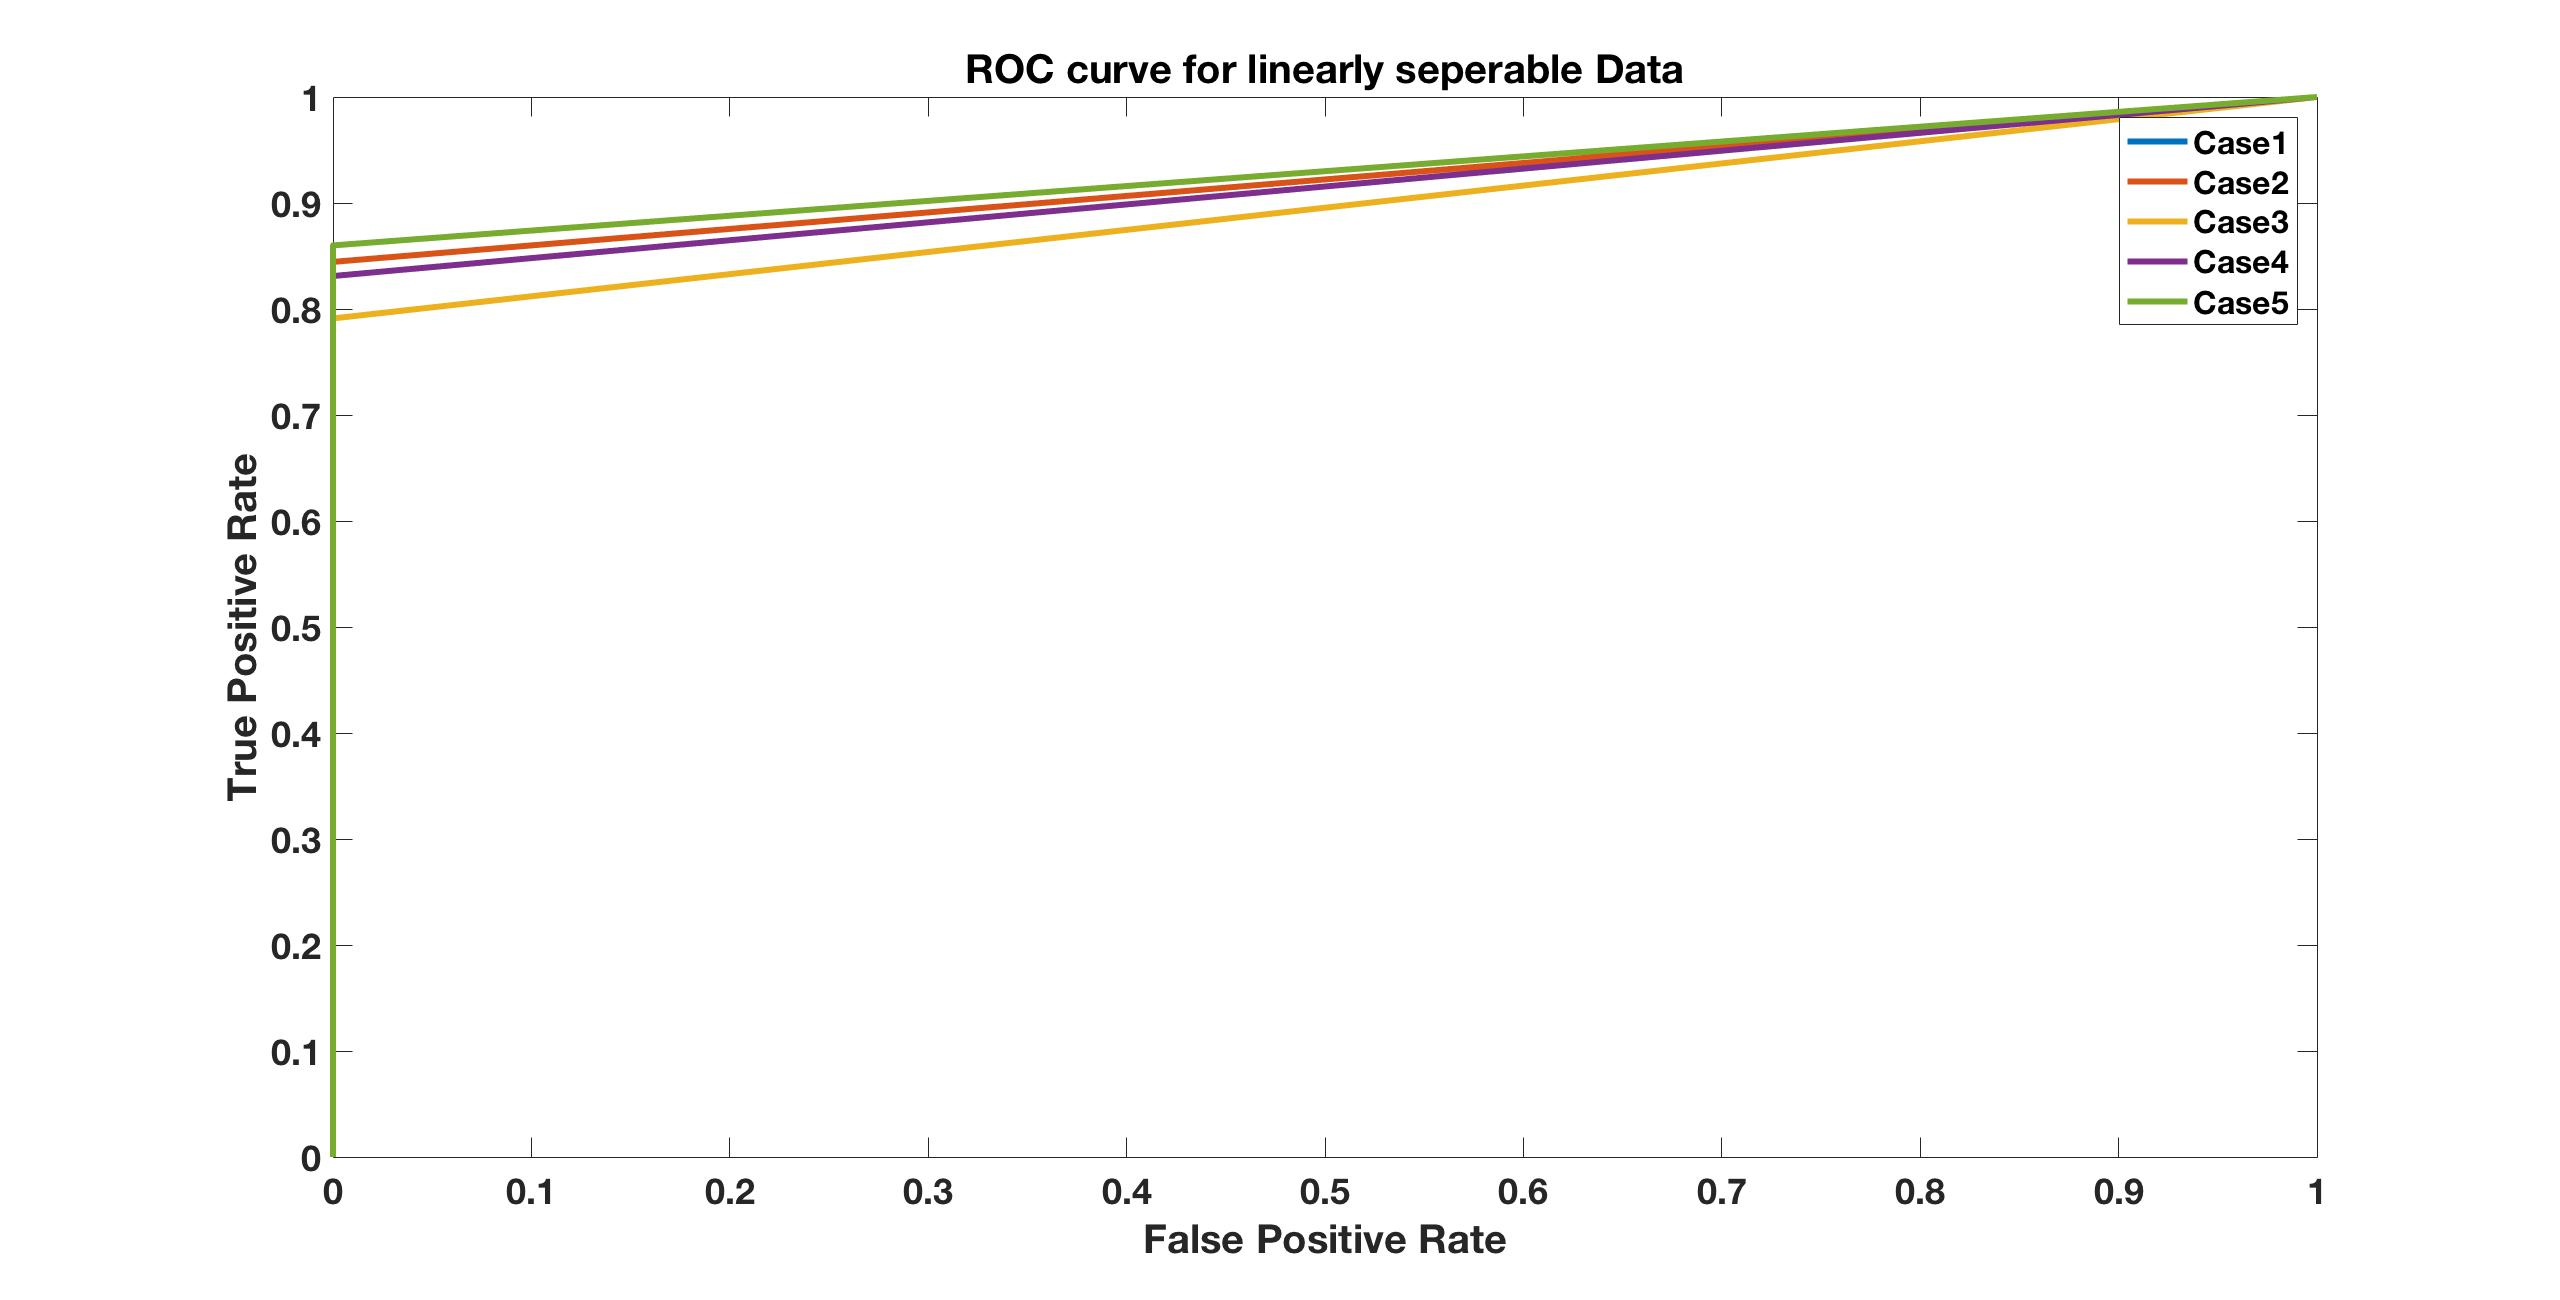
\includegraphics[width=0.7\linewidth]{roc_linear.jpg}
		\end{minipage}\hfill
		\begin{minipage}{1.0\textwidth}
			\centering
			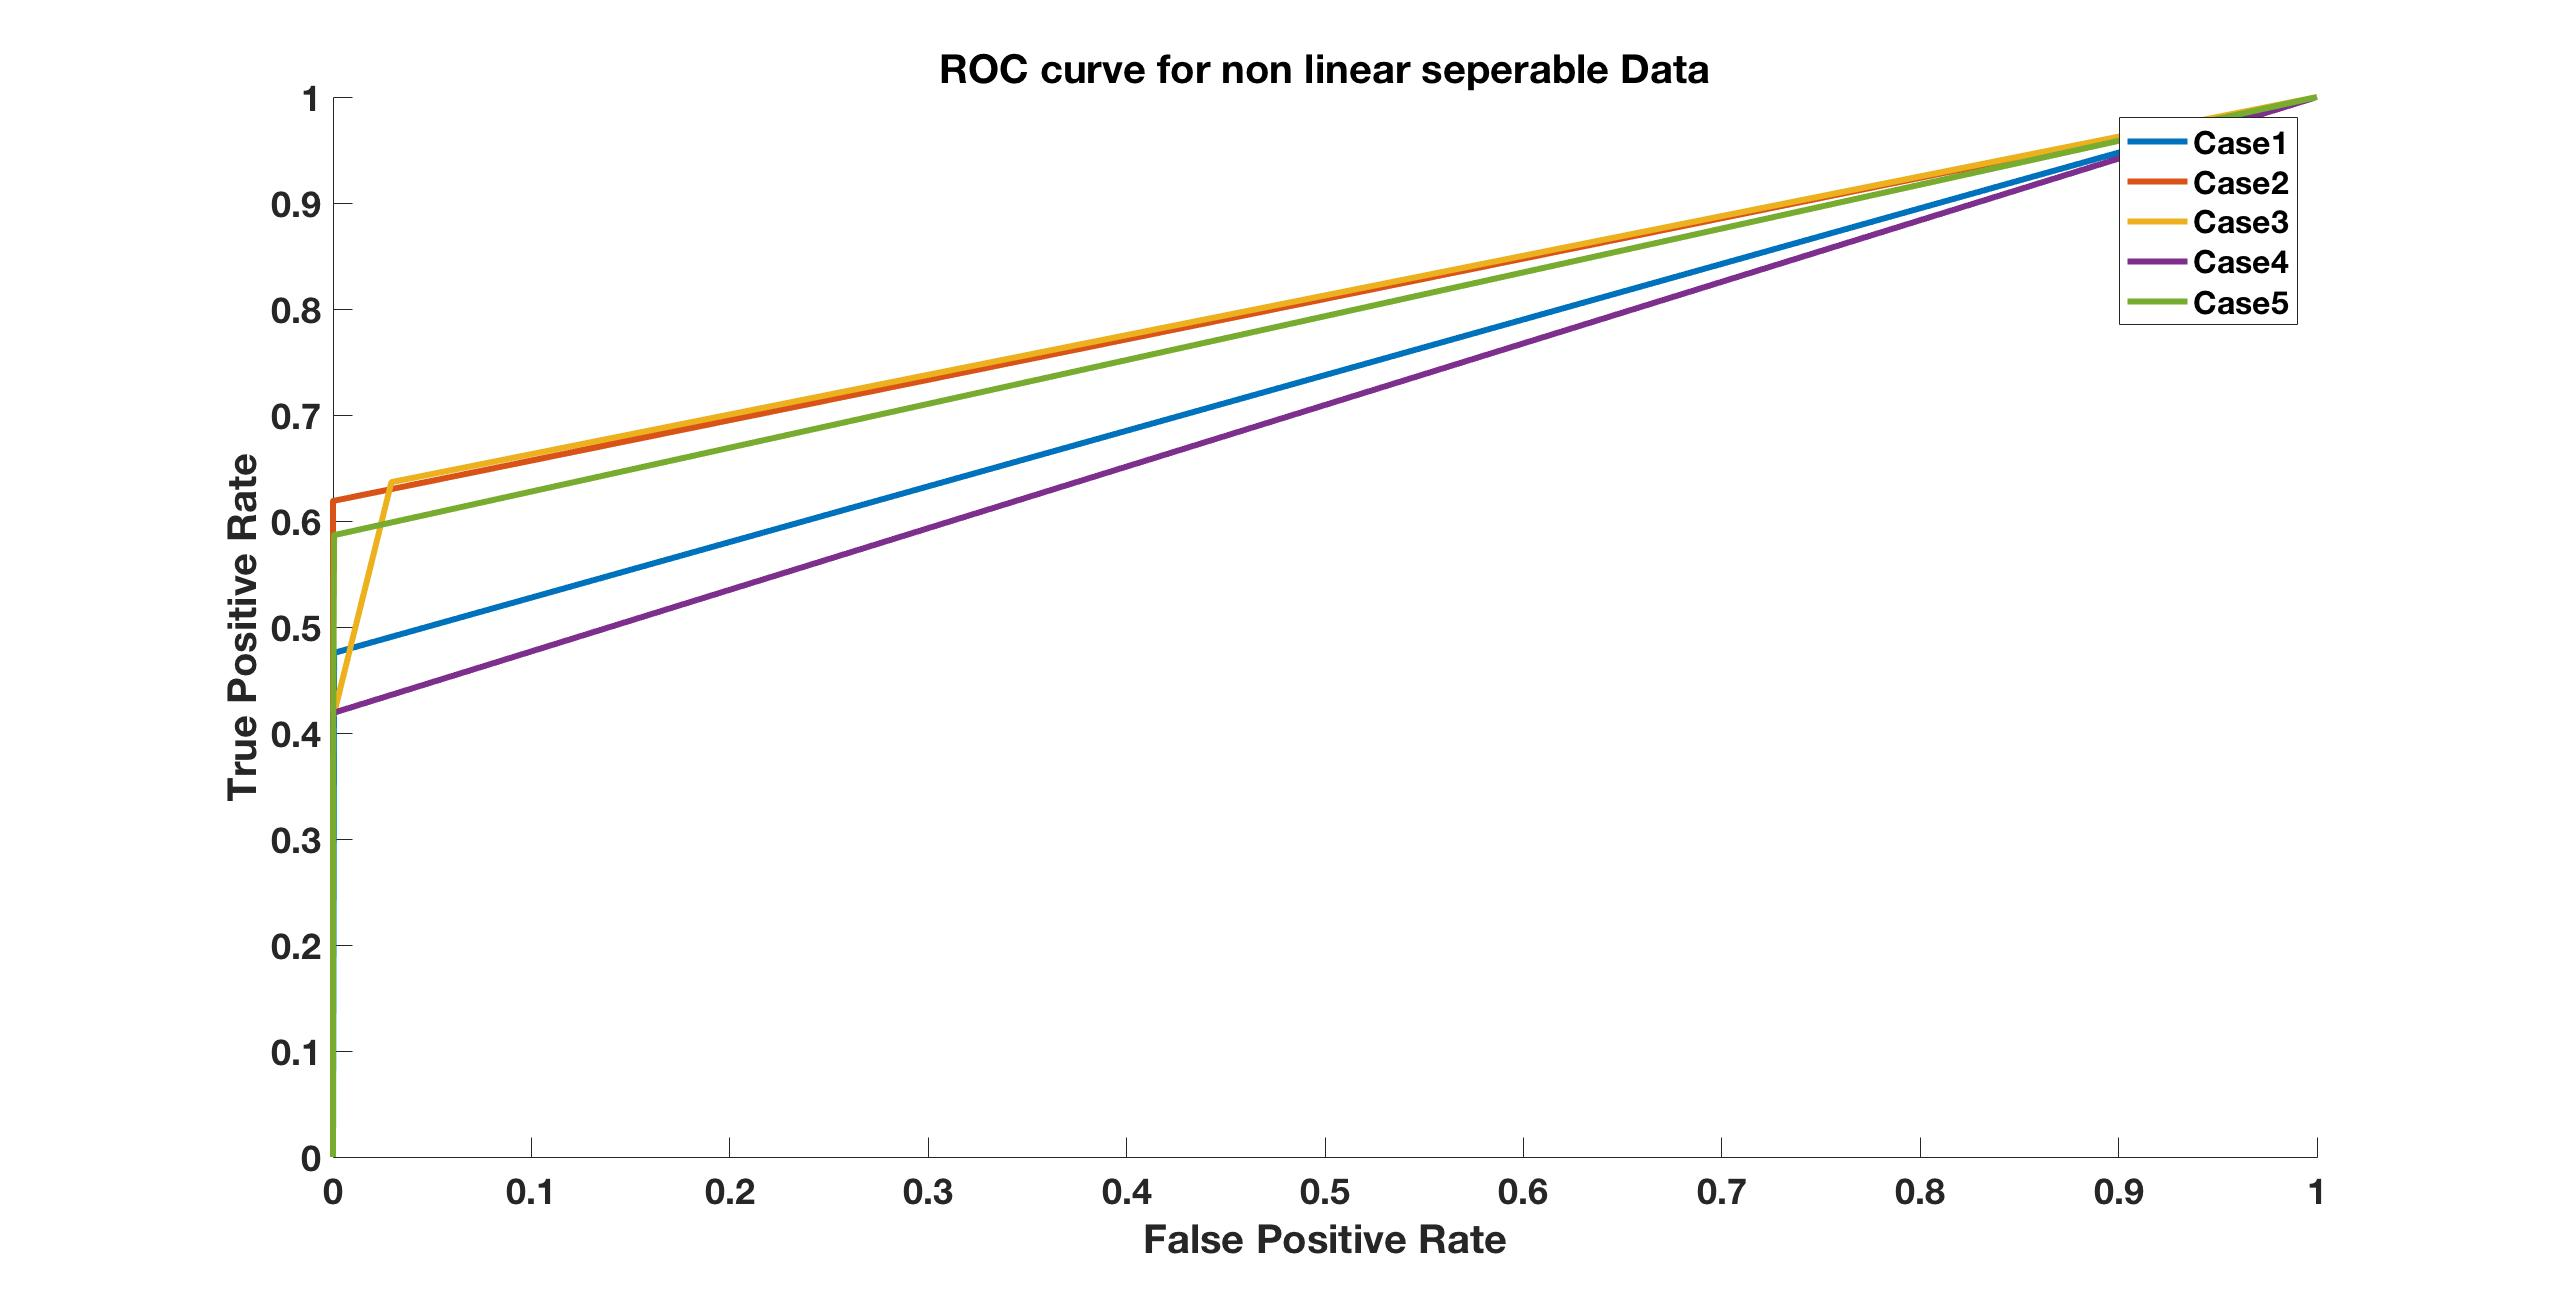
\includegraphics[width=0.7\linewidth]{roc_non_linear.jpg}
		\end{minipage}
		\begin{minipage}{1.0\textwidth}
			\centering
			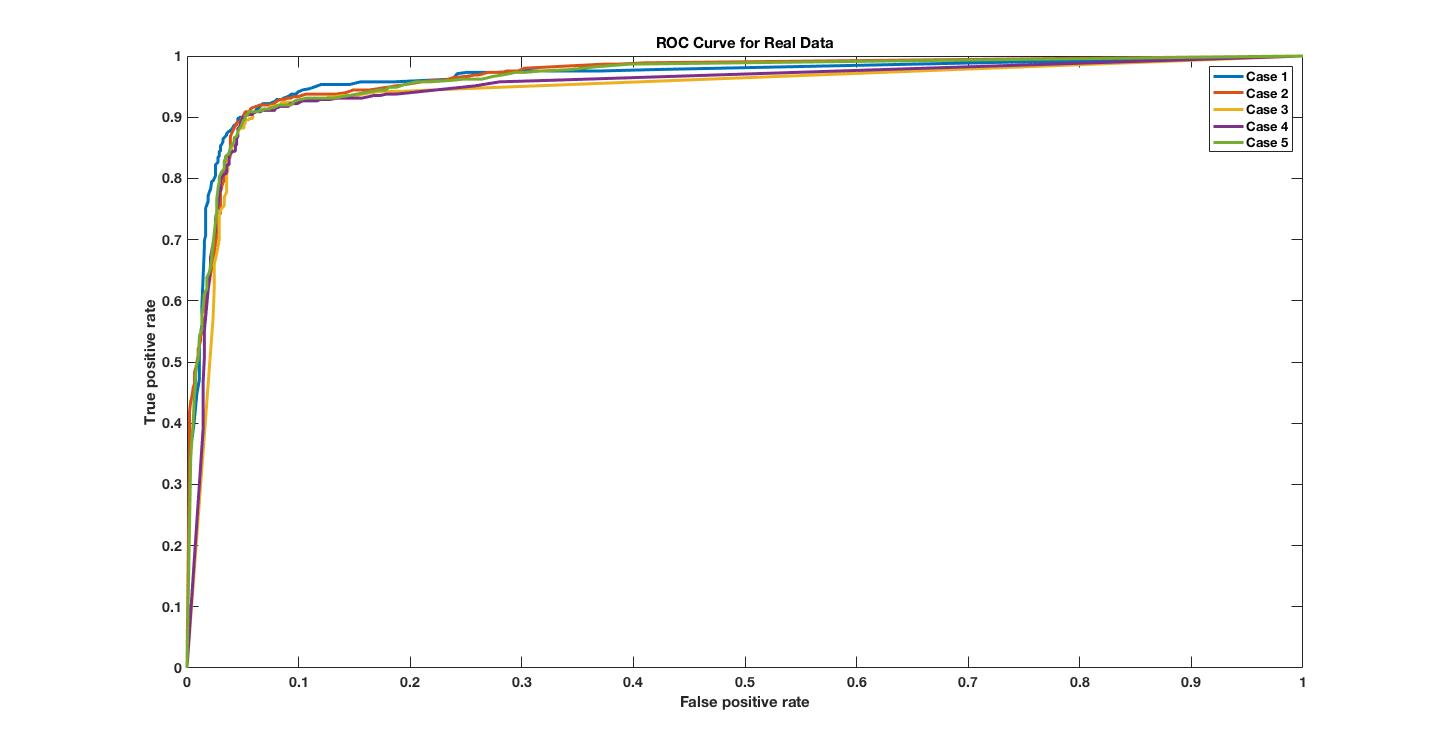
\includegraphics[width=0.7\linewidth]{roc_real.jpg}
		\end{minipage}
	\end{figure}
	ROC curve is plotted for True Positive Rate(TPR) and False Positive Rate(FPR). The model is considered to perform better if goes from origin to top left/right corner and then to diagonal. As our input data becomes more complex our model becomes less effective in prediction and hence our curves tends towards a straight line passing from origin to diagonal.
	
	\section{Detection Error Tradeoff}
	\begin{figure}[H]
		\begin{minipage}{1.0\textwidth}
			\centering
			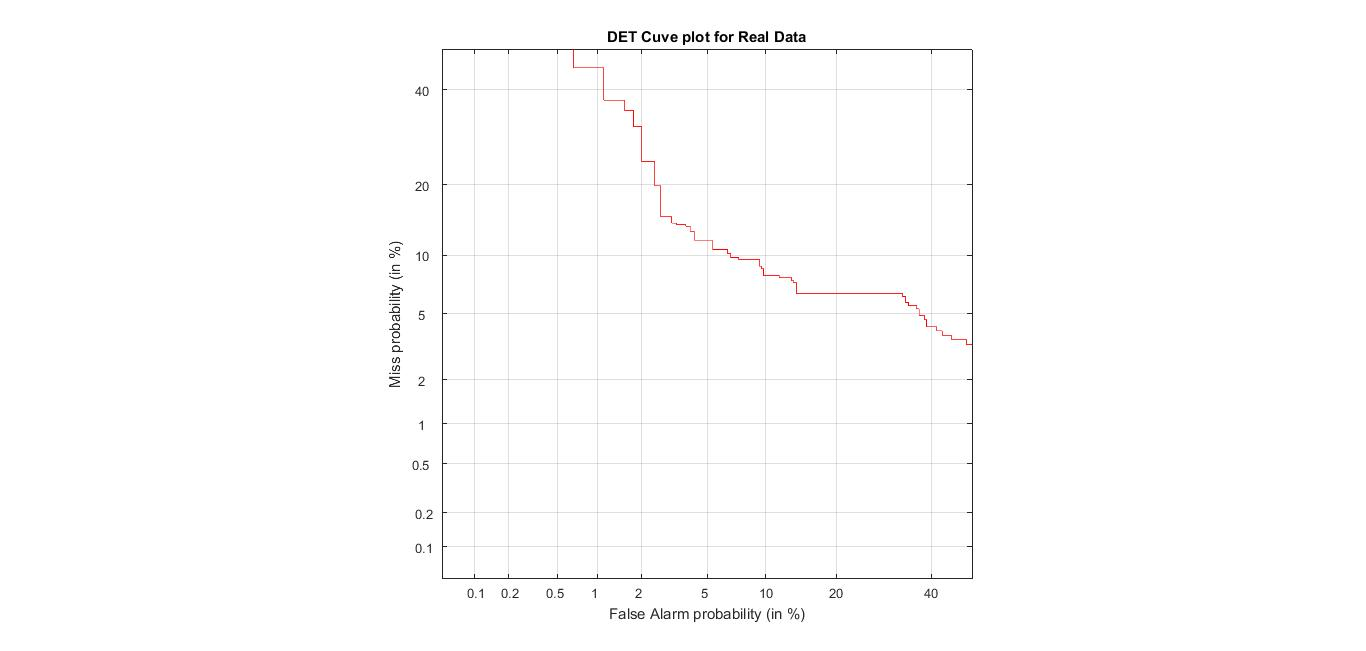
\includegraphics[width=0.9\linewidth]{Det_real.jpg}
		\end{minipage}\hfill
		\begin{minipage}{1.0\textwidth}
			\centering
			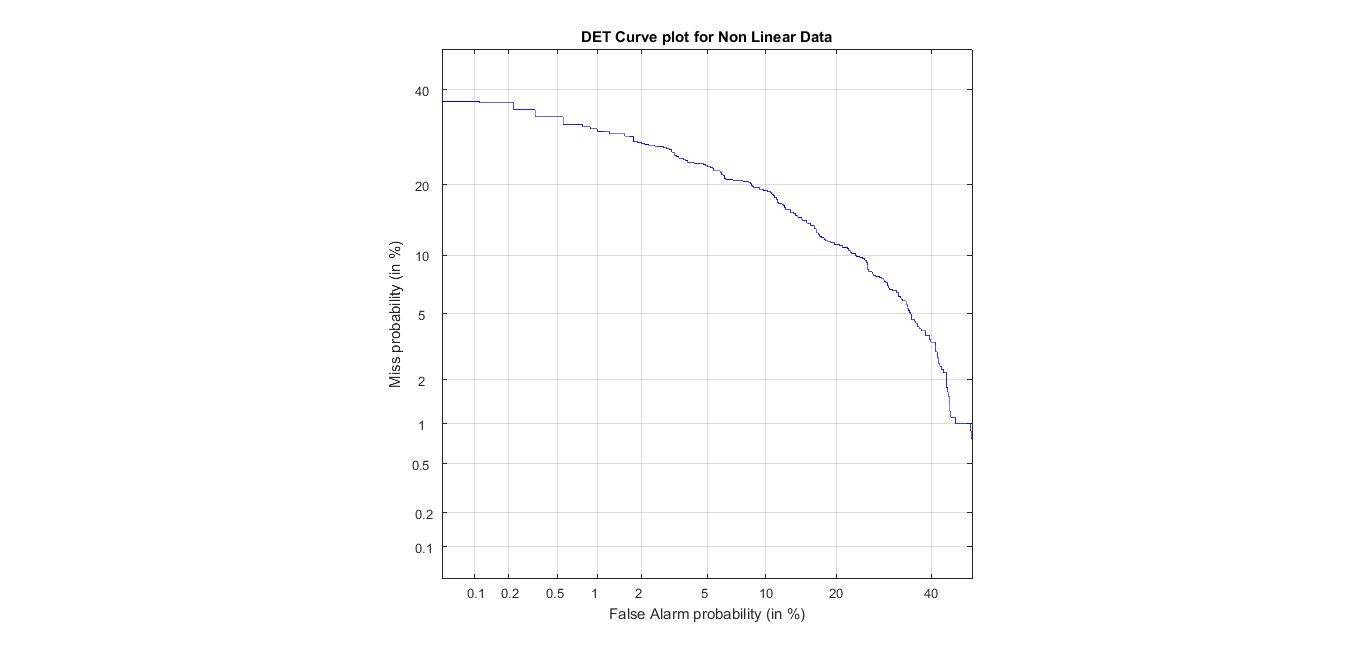
\includegraphics[width=0.9\linewidth]{det_non_lin.jpg}
		\end{minipage}
	\end{figure}
	In DET curve we plot error rates on both axis. Usually plot produces close to linear, for best class system we are closed to left bottom of the plot. The resulting curves are approximately straight line corresponding to normal likelihood distribution.
\end{document}




